\documentclass{beamer}
\usefonttheme{professionalfonts}
\usepackage{lmodern}
\usepackage{ragged2e}
\usepackage[font=small]{caption}
\usepackage{array}
\usepackage{mathtools}
\usepackage{amssymb,amsmath,mathabx}
\usepackage{epstopdf}
\usepackage{graphicx}
\usepackage{amssymb}
\usepackage{appendix}
%\usepackage{enumitem}
%\usepackage{pgf}
\usepackage{caption}
\usepackage{pifont} 
\setbeamertemplate{caption}[numbered]
\usepackage{subcaption}
\captionsetup{compatibility=false}
\usepackage[USenglish]{babel}
\usepackage{wrapfig}
%\usepackage{subfigure}
\usetheme{warsaw}
\usetheme{Copenhagen}
\begin{document}
	\newcommand{\defeq}{\stackrel{\text{def}}{=}}	
	\title[MS Thesis Presentation \hspace{1.2in}\insertframenumber]{MS Thesis Presentation\\Title\\Approximate Solution of Differential Equations using Legendre Wavelet Collocation Method}
	\author[Muhammad Sohaib]{Presented by: Muhammad Sohaib\\ Supervised by: Dr. Sirajul Haq}
	\institute[GIKI]{~~Faculty of Engineering Sciences\\~~Ghulam Ishaq Khan Institute of Engineering Sciences and Technology\\ Topi, Swabi, KPK, Pakistan}
	\date{\today}
	\subject{Informatics}
	%%%%%%%%%%%%%%%%%%%%%%%%%%%%%%%%%%%%%%%%%%%%%%%%
	\frame{\titlepage}
	{\small
		\frame{\frametitle{Presentation Contents}\tableofcontents}
		
	}
	%%%%%%%%%%%%%%%%%%%%%
	%%%%%%%%%%%%%%%%%%%%%
	%%%%%%%%%%%%%%%%%%%%%
\section{Motivation and literature survey}
\frame{ \frametitle{Motivation and literature survay}
\justifying
\begin{itemize}
\item	Differential equations has wide spread applications in science and engineering.
\item	The mathematical model of many real world problems give rise to linear or nonlinear differential equations.
\item	There are different techniques available for the solution of differential equation.
\item	Each technique has its own advantages and limitations.
\item	Exact solution of differential equations in most cases is not easy particularly when the problem is nonlinear.
\item	Therefore, researchers are in progress to develop new methods for the solution of differential equations.	
\end{itemize}
}
	%%%%%%%%%%%%%%%%%%%
	%%%%%%%%%%%%%%%%%%%
	%%%%%%%%%%%%%%%%%%%
	\begin{frame}\frametitle{Motivation and literature survey}
		\begin{itemize}
			\justifying
		 \item	Recently the use of wavelet analysis for the solution of differential equations is very popular.
		 \item	Several wavelet based numerical methods are available in literature for the solution of differential equations.	
		 \item    These methods include Haar Wavelet Method (HWM), Wavelet Finite Element Method (WFEM), Wavelet Meshless  Method (WMM), Wavelet Boundary Element Method (WBEM), Lagrangian Wavelet Method (LWM), Chebyshev Wavelet Method (CWM), and Legendre Wavelet Collocation Method (LWCM)\cite{P1,P2,P3,P4}.
		\end{itemize}
	\end{frame}
%%%%%%%%%%%%%%%%%%%%%
%%%%%%%%%%%%%%%%%%%%%
%%%%%%%%%%%%%%%%%%%%%	
	\section{Legendre Wavelet Collocation Method (LWCM)}
	\begin{frame}\frametitle{Legendre Wavelet Collocation Method (LWCM)}
\begin{itemize}	
	\justifying		
\item Legendre Wavelet Collocation Method (LWCM) is a wavelet based method which uses Legendre polynomials for the solution of differential equations.	
\end{itemize}
\end{frame}
%%%%%%%%%%%%%%%%%%%%%
%%%%%%%%%%%%%%%%%%%%%
%%%%%%%%%%%%%%%%%%%%%
\subsection*{Legendre polynomials and its properties}
\begin{frame}\frametitle{Legendre polynomials and its properties}
\begin{itemize}
	\justifying
\item The use of orthogonal polynomials in approximation theory has gained much consideration. 
\item These polynomials can approximate a function.	
\item The Legendre polynomials $L_{n}(x)$ satisfies the Legendre differential equation which is given by
\begin{eqnarray}
(1-x^2)y''(x)-2xy'(x)+n(n+1)y(x)=0
\end{eqnarray}
where $n$ is non-negative integer.
\end{itemize}
\end{frame}
%%%%%%%%%%%%%%%%%%%%
%%%%%%%%%%%%%%%%%%%%
%%%%%%%%%%%%%%%%%%%%		
\begin{frame}\frametitle{Legendre polynomials and its properties}
	\begin{itemize}
		\justifying
		\item	The Legendre polynomials is given by the following equation \cite{Alexendre}	
	\begin{eqnarray}
		L_n(x)=\sum _{s=0}^{\lfloor\frac{n}{2}\rfloor}\frac{(-1)^s (2 n-2 s)! x^{n-2 s}}{2^n s! (n-s)! (n-2 s)!},
		\end{eqnarray}	
%	where $\lfloor\frac{n}{2}\rfloor$ is the greatest integer not exceeding $\frac{n}{2}$.
	\item Another representation of Legendre polynomials is given by \cite{Alexendre}
	\begin{eqnarray}\label{Leg1}
	L_n(x)=\frac{1}{2^n n!}{\frac{d^n}{dx^n}}(x^2-1)^n,~~~~n=0,1,2,3,\text{...}\text{..}.
	\end{eqnarray}
	Formula (\ref{Leg1}) is known as \emph{Rodrigues} formula. 
	\end{itemize}
\end{frame}
%\subsection{Properties of Legendre polynomials}
%%%%%%%%%%%%%%%%%%%%%%%
%%%%%%%%%%%%%%%%%%%%%%%
%%%%%%%%%%%%%%%%%%%%%%%
\begin{frame}\frametitle{Legendre polynomials and its properties}
	\begin{itemize}	
		\justifying
\item The Legendre polynomials are orthogonal over $[-1, 1]$ i.e.,
\begin{eqnarray}
\int_{-1}^1 L_{n}(x) L_{m}(x) \, dx=\left\{
\begin{array}{ll}
0, & \hbox{$n \neq m$;} \\
\frac{2}{2n+1}, & \hbox{$n=m$}
\end{array}
\right.
\end{eqnarray}
so the set
\begin{eqnarray}
\mu _n(x)=\left\{\sqrt{ n+\frac{1}{2}}L_n(x)\right\},\nonumber
\end{eqnarray}
\small
form an orthonormal set.
\end{itemize}
\end{frame}	
%%%%%%%%%%%%%%%%%%%%
%%%%%%%%%%%%%%%%%%%%
%%%%%%%%%%%%%%%%%%%%
\subsection{Wavelet and Legendre wavelet}
\begin{frame}\frametitle{Wavelet and Legendre wavelet}
	\begin{itemize}
		\justifying
	\item \textbf{Wavelet} means a small wave. Wavelets are mathematical functions that arise in mathematics, quantum physics and engineering. 
	\item \textbf{Legendre wavelets} are constructed from Legendre polynomial. Legendre wavelets $\psi_{n,m}(x)=\psi(k,n,m,x)$ have four arguments, $k$ and $n$ are positive integers, $m$ is the order of Legendre polynomials. The Legendre wavelet \cite{Razaghi} is defined on $[0,1]$ by
	\small	
	\begin{eqnarray}
	\psi_{n,m}(x)=\left\{
	\begin{array}{ll}
	\sqrt{m+\frac{1}{2}}~2^{\frac{k}{2}}~L_{m}(2^{k}x-2n+1), & \hbox{$\frac{n-1}{2^{k-1}} \leq x \leq\frac{n}{2^{k-1}} $;} \\
	0, & \hbox{Otherwise}
	\end{array}
	\right.
	\end{eqnarray}
	\normalsize	
	\end{itemize}
\end{frame}
%%%%%%%%%%%%%%%%%%%%
%%%%%%%%%%%%%%%%%%%%
%%%%%%%%%%%%%%%%%%%%
\begin{frame}\frametitle{Wavelet and Legendre wavelet}
	\justifying
	where $n=1,2,3.........2^{k-1}$, $m=0,1,2,3,.........M-1$, the coefficients $\sqrt{m+\frac{1}{2}}$ are for orthonormality. $M$ determines the order or level of the wavelet.
	%\begin{itemize}
	$L_{m}(x)$ are the Legendre polynomials of order $m$ which are defined on the interval [-1, 1] and are given by the following recurrence relations,
	\begin{align}
	L_{0}(x)=1,\nonumber\\
	L_{1}(x)=x,\nonumber
	\end{align}
	\small
	\begin{eqnarray}
	L_{m+1}(x)=\left(\frac{2m+1}{m+1}\right)~x~L_{m}(x)-\left(\frac{m}{m+1}\right)~L_{m-1}(x),~m=1,2,3...\nonumber
	\end{eqnarray}
	\small
	\begin{itemize}
	\item The Legendre wavelet form an orthonormal basis for $L^{2}(R)$ \cite{Khellat,Razaghi,Raz}.
\end{itemize}
\end{frame}
%%%%%%%%%%%%%%%%%%
%%%%%%%%%%%%%%%%%%
%%%%%%%%%%%%%%%%%%
\subsection{Description of LWCM}
\begin{frame}\frametitle{Description of LWCM}
	%\begin{itemize}
		\justifying
	%	\begin{block}{Consider the following BVP of order $n$}
	 Consider the following IBVP of order $n$
		\begin{eqnarray}\label{ch4}
			u^{(n)}(x)=f(x, u(x), u'(x), .....,u^{(n-1)}(x)),~~~~~a\leq x \leq b,
			\end{eqnarray}
			\small
			subject to the following initial and boundary conditions\\
	\textbf{Case (i)}
	\begin{eqnarray}\label{cha}
		u^{(j-1)}(a)=A_{j},~~~~~~j=1, 2, 3,.....,n.
	\end{eqnarray}
\textbf{Case (ii)}
	\begin{eqnarray}\label{chb}
		u^{(j-1)}(a)=A_{j},~~~u^{(j-1)}(b)=B_{j},~~~~~j=1, 2, 3,.....,\frac{n}{2}.
	\end{eqnarray}
\textbf{Case (iii)}
	\begin{eqnarray}\label{chc}
		u^{(j-2)}(a)=A_{j},~~~u^{(j-2)}(b)=B_{j},~~~~~j=2, 4, 6,.....,n.
	\end{eqnarray}
	 \end{frame}
%%%%%%%%%%%%%%%%%%%%
%%%%%%%%%%%%%%%%%%%%
%%%%%%%%%%%%%%%%%%%%	    	
	\begin{frame}\frametitle{Description of LWCM}
		\justifying
	    Where $n=2, 4, 6, 8, 10,12$, $A_{j}$ and $B_{j}$ are known constants while $u(x)$ is unknown function to be determined. According to LWCM
		\begin{eqnarray}\label{ch5}
		u(x)=\sum_{n=1}^{2^{k-1}}\sum_{m=0}^{M-1}s_{n,m}\psi_{n,m}(x)=S^{T}\psi(x),
		\end{eqnarray} 
	    where $S$ and $\psi(x)$ are $2^{k-1}M\times1$ matrices given by
		\begin{eqnarray}\label{6}
		S=[s_{1,0},...,s_{1,M-1},s_{2,0},...,s_{2,M-1},...,s_{2^{k-1},0},...,s_{2^{k-1},M-1}]^{T},\nonumber
		\end{eqnarray}
		\small
		\begin{eqnarray}\label{7}
		\psi(x)=[\psi_{1,0},...,\psi_{1,M-1},\psi_{2,0},...,\psi_{2,M-1},...,\psi_{2^{k-1},0},...,\psi_{2^{k-1},M-1}]^{T}.\nonumber
		\end{eqnarray}
		\normalsize   	
\end{frame}
%%%%%%%%%%%%%%%%%%
%%%%%%%%%%%%%%%%%%
%%%%%%%%%%%%%%%%%%
\begin{frame}\frametitle{Description of LWCM}
\justifying
	Using Eq. (\ref{ch5}) in Eq. (\ref{ch4}) and Eq. (\ref{cha}) (Case (i)) or Eq. (\ref{chb}) (Case (ii)) or Eq. (\ref{chc}) (Case (iii)) the following equation is obtained
	\begin{eqnarray}\label{ch8}
	S^{T}\psi^{(n)}(x)=f(x,S^{T}\psi(x), S^{T}\psi'(x),...,S^{T}\psi^{(n-1)}(x)),
	\end{eqnarray}
	\small
	\normalsize
	and Eq. ((\ref{cha}) (Case (i)) or Eq. (\ref{chb}) (Case (ii)) or Eq. (\ref{chc}) (Case (iii)) will become
	\begin{align}
	&S^{T}\psi^{(j-1)}(a)=A_{j},~~j=1, 2, 3,.....,n.\label{pak1}\\
	&S^{T}\psi^{(j-1)}(a)=A_{j},~~S^{T}\psi^{(j-1)}(b)=B_{j},~~j=1, 2, 3,...,\frac{n}{2}.\label{pak2}\\
	&S^{T}\psi^{(j-2)}(a)=A_{j},~~S^{T}\psi^{(j-2)}(b)=B_{j},~~j=2, 4, 6,.....,n.\label{pak3}
	\end{align}
	\small
	\normalsize   
\end{frame}
%%%%%%%%%%%%%%%%%%%%
%%%%%%%%%%%%%%%%%%%%
%%%%%%%%%%%%%%%%%%%%
\begin{frame}\frametitle{Description of LWCM}
	\justifying
 From Eq. (\ref{ch5}) it is clear that there are total $2^{k-1}M$  unknown constants. To find these unknown constants one need $2^{k-1}M$ equations. Out of these $2^{k-1}M$ equations $n$ number of equations will be obtained from Eq. (\ref{pak1}) or (\ref{pak2}) or (\ref{pak3}).
  For rest of the equations consider the following collocation points, which are zeros of Chybeshev polynomials \cite{Sadeghi}
  \begin{eqnarray}\label{9}
  x_{i}=\cos\left[\frac{(2i+1)\pi}{2^{k}M}\right], ~~~~~i=1, 2, 3, 4, .....,2^{k-1}M-n.
  \end{eqnarray}
  \small
 Using these collocation points in Eq. (\ref{ch8}) the following equation is obtained
\end{frame}
%%%%%%%%%%%%%%%%%%%%%%
%%%%%%%%%%%%%%%%%%%%%%
%%%%%%%%%%%%%%%%%%%%%%
\begin{frame}\frametitle{Description of LWCM}
\justifying
 \begin{eqnarray}\label{ch10}
 S^{T}\psi^{(n)}(x_{i})=f(x_{i},S^{T}\psi(x_{i}), S^{T}\psi'(x_{i}),...,S^{T}\psi^{(n-1)}(x_{i})).
 \end{eqnarray}
Eq. (\ref{ch10}) together with Eq. (\ref{pak1}) or Eq. (\ref{pak2}) or Eq. (\ref{pak3}) gives a system of ${2^{k-1}M}$ equations. Solution of this system of equations will give the unknown matrix $S$. Using $S$ in Eq. (\ref{ch5}) will give the desire solution.
\end{frame}	
%%%%%%%%%%%%%%%%%%%
%%%%%%%%%%%%%%%%%%%
%%%%%%%%%%%%%%%%%%%
\section{Application of LWCM to ODEs}
\subsection*{Example 1}
\begin{frame}\frametitle{Example 1}
	\justifying
\textbf{Example 1} Consider the nonlinear squeezing flow problem of order four \cite{Idrees}
\begin{eqnarray}\label{ch57}
u^{(4)}(x)+R_{e}u(x)u^{(3)}(x)=0,~~~~0\leq x \leq 1,
\end{eqnarray}
with the boundary conditions
\begin{eqnarray}\label{ch58}
&u(0)=0,~~~~~~~~~u''(0)=0,\nonumber\\
&u(1)=1,~~~~~~~~~u'(1)=0,
\end{eqnarray}
where $R_{e}$ is the Reynold number.\\
Setting $k=1$ and $M=9$ in Eq. (\ref{ch5})
\begin{eqnarray}\label{ch60}
u(x)=\sum_{n=1}^{1}\sum_{m=0}^{8}s_{n,m}\psi_{n,m}(x)=S^{T}\psi(x),
\end{eqnarray}	
\end{frame}
%%%%%%%%%%%%%%%%%%
%%%%%%%%%%%%%%%%%%
%%%%%%%%%%%%%%%%%%
\begin{frame}\frametitle{Example 1}
\justifying
where $S$ and $\psi(x)$ are given by
\begin{align}
&S=[s_{1,0}, s_{1,1}, .....,s_{1,8}]^{T},\nonumber\\
&\psi(x)=[\psi_{1,0}, \psi_{1,1}, .....,\psi_{1,8}]^{T}.\nonumber
\end{align}
\small
Now using Eq. (\ref{ch60}) in Eq. (\ref{ch57}) and (\ref{ch58}) the following equations are obtained
\begin{eqnarray}\label{ch61}
S^{T}\psi^{(4)}(x)+R_{e}S^{t}\psi(x)S^{T}\psi^{(3)}(x)=0.
\end{eqnarray}
\small
%with the conditions
\begin{eqnarray}\label{ch62}
&S^{T}\psi(0)=0,~~~~~~~~~S^{T}\psi''(0)=0,\nonumber\\
&S^{T}\psi(1)=1,~~~~~~~~~S^{T}\psi'(1)=0.
\end{eqnarray}
\small
The equations obtained from Eq. (\ref{ch62}) in case of $R_{e}=1$ are given by
\end{frame}
%%%%%%%%%%%%%%%%%%%
%%%%%%%%%%%%%%%%%%%
%%%%%%%%%%%%%%%%%%%
\begin{frame}\frametitle{Example 1}
	\justifying
	\tiny
\begin{eqnarray}\label{ch62a}
&s_{1,0}-\sqrt{3}s_{1,1}+\sqrt{5}s_{1,2}-\sqrt{7}s_{1,3}+3s_{1,4}-\sqrt{11}s_{1,5}+\sqrt{13}s_{1,6}-\nonumber\\
&\sqrt{15}s_{1,7}+\sqrt{17}s_{1,8}=0.
\end{eqnarray}
\tiny
\begin{eqnarray}\label{ch62b}
&12\sqrt{5}s_{1,2}-60\sqrt{7}s_{1,3}+540s_{1,4}-420\sqrt{11}s_{1,5}+840\sqrt{13}s_{1,6}-1512\sqrt{15}s_{1,7}+\nonumber\\
&2520\sqrt{17}s_{1,8}=0.
\end{eqnarray}
\tiny
\begin{eqnarray}\label{ch62c}
&s_{1,0}+\sqrt{3}s_{1,1}+\sqrt{5}s_{1,2}+\sqrt{7}s_{1,3}+3s_{1,4}+\sqrt{11}s_{1,5}+\sqrt{13}s_{1,6}+\sqrt{15}s_{1,7}+\nonumber\\
&\sqrt{17}s_{1,8}=1.
\end{eqnarray}
\tiny
\begin{eqnarray}\label{ch62d}
&2\sqrt{3}s_{1,1}+6\sqrt{5}s_{1,2}+12\sqrt{7}s_{1,3}+60s_{1,4}+30\sqrt{11}s_{1,5}+42\sqrt{13}s_{1,6}+56\sqrt{15}s_{1,7}+\nonumber\\
&72\sqrt{17}s_{1,8}=0.
\end{eqnarray}		
\end{frame}
%%%%%%%%%%%%%%%
%%%%%%%%%%%%%%%
%%%%%%%%%%%%%%%
\begin{frame}\frametitle{Example 1}
\justifying
Now collocating Eq. (\ref{ch61}) at $x_{i}$, which are zeros of of chebyshev polynomials, the following equation is obtained
\begin{eqnarray}\label{ch63}
S^{T}\psi^{(4)}(x_{i})+R_{e}S^{t}\psi(x_{i})S^{T}\psi^{(3)}(x_{i})=0\nonumber,
\end{eqnarray}
which gives the following equations
\tiny
\begin{equation}\label{ch63aa}
\begin{aligned}
&5040s_{1,4}+48623.66446s_{1,5}+254635.662s_{1,6}+959983.48s_{1,7}+2.915216\times10^{6}s_{1,8}+\\
&(1.000000000s_{1,0}+1.6794233s_{1,1}+2.0353392s_{1,2}+2.1815464s_{1,3}+\\
&2.1493208s_{1,4}+1.9593666s_{1,5}+1.6338131s_{1,6}+1.1990648s_{1,7}+\\
&0.68592302s_{1,8}) (120 \sqrt{7}s_{1,3}+2443.431075s_{1,4}+10393.5823s_{1,5}+ \\
&32339.865s_{1,6}+82161.54s_{1,7}+180465.8s_{1,8})=0.
\end{aligned}
\end{equation}
\end{frame}
%%%%%%%%%%%%%
%%%%%%%%%%%%%
%%%%%%%%%%%%%
\begin{frame}\frametitle{Example 1}
	\justifying
	\tiny
\begin{equation}\label{ch63bb}
\begin{aligned}
&5040s_{1,4}+36710.42039s_{1,5}+133424.542s_{1,6}+311750.48s_{1,7}+491497.9s_{1,8}+\\
&(1.000000000s_{1,0}+1.26794919s_{1,1}+0.67942384s_{1,2}-0.310383928s_{1,3}-\\
&1.134526419s_{1,4}-1.341466309s_{1,5}-0.820935633s_{1,6}+0.1438470268s_{1,7}+\\
&1.031623756s_{1,8}) (120 \sqrt{7}s_{1,3}+1844.768035s_{1,4}+5325.4908s_{1,5}+\\
&9627.518s_{1,6}+10612.03s_{1,7}+2791.8s_{1,8})=0.
\end{aligned}
\end{equation}
\normalsize
%\end{gather}
%\begin{gather}
\tiny
\begin{equation}\label{ch63cc}
\begin{aligned}
&5040s_{1,4}+14320.84528s_{1,5}-2805.247s_{1,6}-59472.77s_{1,7}-58981.2s_{1,8}+\\
&(1.000000000s_{1,0}+0.494630789s_{1,1}-0.844496220s_{1,2}-0.979295460s_{1,3}+\\
&0.294819829s_{1,4}+1.149631888s_{1,5}+0.359054432s_{1,6}-0.946147563s_{1,7}-\\
&0.898606254s_{1,8}) (120 \sqrt{7}s_{1,3}+719.649553s_{1,4}-\\
&370.56278s_{1,5}-2728.2515s_{1,6}-1746.33s_{1,7}+4647.00s_{1,8})=0.
\end{aligned}
\end{equation}
\normalsize
%%%%%%
\tiny
\begin{equation}\label{ch63dd}
\begin{aligned}
&5040s_{1,4}-15844.54765s_{1,5}+2674.9864s_{1,6}+57740.682s_{1,7}-81244.40s_{1,8}+\\
&(1.000000000s_{1,0}-0.547258277s_{1,1}-0.783192177s_{1,2}+1.045292682s_{1,3}+\\
&0.1327119654s_{1,4}-1.131717877s_{1,5}+0.579750401s_{1,6}+0.767347457s_{1,7}-\\
&1.064052468s_{1,8}) (120\sqrt{7}s_{1,3}-796.218478s_{1,4}-\\
&141.42273s_{1,5}+2729.9419s_{1,6}-2639.641s_{1,7}-3579.97s_{1,8})=0.
\end{aligned}
\end{equation}
\normalsize
\end{frame}
%%%%%%%%%%%%%%
%%%%%%%%%%%%%%
%%%%%%%%%%%%%%	
\begin{frame}\frametitle{Example 1}
	\justifying
\begin{equation}\label{ch63ee}
\tiny
\begin{aligned}
&5040s_{1,4}-15120 \sqrt{11} s_{1,5}+75600 \sqrt{13} s_{1,6}-277200 \sqrt{15} s_{1,7}+831600 \sqrt{17} s_{1,8}+\\
&(s_{1,0}-\sqrt{3} s_{1,1}+\sqrt{5} s_{1,2}-\sqrt{7} s_{1,3}+3 s_{1,4}-\sqrt{11} s_{1,5}+\sqrt{13} s_{1,6}-\sqrt{15} s_{1,7}+\\
&\sqrt{17} s_{1,8})(120 \sqrt{7} s_{1,3}-2520 s_{1,4}+3360 \sqrt{11} s_{1,5}-10080 \sqrt{13} s_{1,6}+25200 \sqrt{15} s_{1,7}-\\
&55440 \sqrt{17} s_{1,8})=0.\\
\end{aligned}
\end{equation}
Solving the system of equations (\ref{ch62a}-\ref{ch63ee}), the values of unknown constants are obtained which are
\begin{align}
 &s_{1,0}= 0.63023, s_{1,1}=0.30223, s_{1,2}=-0.058734,\nonumber\\ &s_{1,3}=-0.0088964, s_{1,4}= 0.00037135, s_{1,5}=0,\nonumber\\ &s_{1,6}=0, s_{1,7}=0, s_{1,8}=0.\nonumber
 \end{align}
  Using these constants in Eq. (\ref{ch60}) the solution can be found. Numerical results and comparison with OHAM for different Reynolds numbers are given in Table \ref{chT8}.	
\end{frame}	
%%%%%%%%%%%%%%
%%%%%%%%%%%%%%	
\begin{frame}\frametitle{Example 1}
	\justifying
\begin{figure}[h]
	\centering
	\includegraphics[width=0.9\textwidth]{squ2.eps}\\
	\caption{Plot for different values of $R_{e}$}\label{chF8}
\end{figure}
\end{frame}
%%%%%%%%%%%%%
%%%%%%%%%%%%%
\begin{frame}\frametitle{Example 1}
	\justifying
	%\small
\begin{center}
	\captionof{table}{\footnotesize Comparison of LWCM solution with OHAM solution of Example 1 for $k=1$ and $M=9$ \cite{Idrees}}\label{chT8}
	\scalebox{0.65}{
		\begin{tabular}{l l l l l l l l l}
			\hline
			\multicolumn{1}{l}{$x_{i}$} &
			\multicolumn{2}{p{3cm}}{\centering$R_{e}=1$}&
			\multicolumn{2}{p{3cm}}{\centering$R_{e}=3$}&
			\multicolumn{2}{p{3cm}}{\centering$R_{e}=4$}&
			\multicolumn{2}{p{3cm}}{\centering$R_{e}=10$} \\
			\cline{2-9}\\
			& OHAM & LWCM & OHAM &LWCM&OHAM&LWCM&OHAM&LWCM\\
			\hline
			0.00 &0.000000& $7.4\times10^{-5}$&0.000000 &0.000000&0.000000&$-1.1\times10^{-4}$&0.000000 &$2.8\times10^{-5}$\\
			%\hline
			0.15 & 0.227784 & 0.227946 & 0.235947 & 0.236053& 0.239637& 0.239530& 0.256306 & 0.252730\\
			%\hline
			0.30 &0.444185&0.444507 &0.457974 &0.457991&0.464078&0.463518 &0.489628 &0.483890\\
			%\hline
			0.45 &0.638166 &0.638488 &0.653380 & 0.653183 &0.659864&0.658960 &0.683059& 0.678679\\
			%\hline
			0.60 &0.799349& 0.799565& 0.811634 &0.811380&0.816571& 0.815828& 0.829301&0.829440\\
			%\hline
			0.75 & 0.918249&0.918365&0.924870 &0.924714& 0.927305&0.926966&0.929652 &0.933226\\
			%\hline
			0.90 &0.986419&0.986460&0.987774 & 0.987701&0.988210&0.988087&0.987436 & 0.989344\\
			\hline
		\end{tabular}}
	\end{center}
	\small
	\normalsize
	%\include{}
\end{frame}
%%%%%%%%%%%%%%
%%%%%%%%%%%%%%
%%%%%%%%%%%%%%
%%%%%%%%%%%%%%%%%%
%%%%%%%%%%%%%%%%%%
%%%%%%%%%%%%%%%%%%
\subsection*{Example 2}
\begin{frame}\frametitle{Example 2}
	\justifying
\textbf{Example 2} Consider nonlinear eight order IVP \cite{Raju}
\begin{eqnarray}\label{ch92}
u^{(8)}(x)=e^{-x}u^{2}(x),~~0<x<1,
\end{eqnarray}
\small
with the initial conditions
\begin{align}\label{chsoh9}
& u(0)=1, u'(0)=1,\nonumber\\
&u''(0)=1, u^{(3)}(0)=1,\\
&u^{(4)}(0)=1, u^{(5)}(0)=1,\nonumber\\
&u^{(6)}(0)=1, u^{(7)}(0)=1.\nonumber
\end{align}
\small
Exact solution of Eq. (\ref{ch92}) is \cite{Raju}
\begin{eqnarray}\label{ch93}
u(x)=e^{x}
\end{eqnarray}
\small
The given problem was solved for $k=1$, $M=12$ with the help of LWCM. The results obtained are given in Table \ref{chT19}.
\end{frame}
%%%%%%%%%%%%%%%%%
%%%%%%%%%%%%%%%%%
%%%%%%%%%%%%%%%%%
%%%%%%%%%%%%%%%%%%%%%%
%%%%%%%%%%%%%%%%%%%%%%
%%%%%%%%%%%%%%%%%%%%%%
\begin{frame}\frametitle{Example 2}
	\justifying
\begin{center}
	\captionof{table}{\footnotesize Comparison of absolute error of Example 2 for $k=1$ and $M=12$.}\label{chT19}
	\scalebox{0.70}{
		\begin{tabular}{c c c c c}
			\hline
			\textbf{$x_{i}$}&\textbf{Exact}&\textbf{Approximate}&\textbf{Absolute error (LWCM)}&\textbf{QBS} \cite{Raju}\\
			\hline
			0.1&1.1051709180756477                    &1.1051709180756477               &0.000000000000&$1.192093\times10^{-7}$\\
			%\hline
			0.2&1.2214027581601699                    &1.2214027581602247          &$5.48450\times10^{-14}$&$1.251698\times10^{-5}$\\
			%\hline
			0.3&1.3498588075760032                   &1.3498588075774163              &$1.41309\times10^{-12}$&$4.529953\times10^{-5}$\\
			%\hline
			0.4&1.4918246976412703                    &1.4918246976552993               &$1.40290\times10^{-11}$&$8.225441\times10^{-5}$\\
			%\hline
			0.5&1.6487212707001282                   &1.648721270782562             &$8.24338\times10^{-11}$&$1.045465\times10^{-4}$\\
			%\hline
			0.6&1.8221188003905089                    &1.8221188007377276                 &$3.47219\times10^{-10}$&$9.799004\times10^{-5}$\\
			%\hline
			0.7&2.0137527074704766                &2.0137527086321660                   &$1.16169\times10^{-9}$&$6.628036\times10^{-5}$\\
			%\hline
			0.8&2.2255409284924680                 &2.2255409317757855              &$3.28332\times10^{-9}$&$3.147125\times10^{-5}$\\
			%\hline
			0.9&2.4596031111569500                    &2.4596031193152610           &$8.15831\times10^{-9}$&$1.168251\times10^{-5}$\\
			\hline
		\end{tabular}}
	\end{center}
	\normalsize
\end{frame}
%%%%%%%%%%%%%%%%
%%%%%%%%%%%%%%%%
%%%%%%%%%%%%%%%%
\subsection*{Example 3}
\begin{frame}\frametitle{Example 3}
\textbf{Example 3} Consider the nonlinear twelfth order BVP\cite{DTM1}
\begin{eqnarray}\label{125}
u^{(12)}(x)=2e^{x}u^{2}(x)+u^{(3)}(x),~~~~0<x<1,
\end{eqnarray}
subject to the boundary conditions:
\begin{eqnarray}\label{126}
u^{(2s)}(0)=1,~~~~~u^{(2s)}(1)=e^{-1},~~~~s=0(1)5.
\end{eqnarray}
Exact solution of Eq. (\ref{125}) is\cite{DTM1}
\begin{eqnarray}\label{127}
u(x)=e^{-x}.
\end{eqnarray}
For $k=1$ and $M=18$ the numerical results are given in Table \ref{T27}
\end{frame}
\begin{frame}\frametitle{Example 3}
	\justifying
\begin{center}
	\captionof{table}{\footnotesize Comparison of absolute error of Example 3 for $k=1$ and $M=18$.}\label{T27}
	\scalebox{0.70}{
		\begin{tabular}{c c c c c}
			\hline
			\textbf{$x_{i}$}&\textbf{Exact}&\textbf{Approximate}&\textbf{Absolute error (LWCM)}&\textbf{DTM} \cite{DTM1}\\
			\hline
			0   &           1.0000000000000000                                       &0.9999999999999996                &$4.44089\times10^{-16}$&0.000000000\\
			%\hline
			0.1&0.9048374180359595                    &0.9048374181017839                   &$6.58243\times10^{-11}$&$-1.61\times10^{-7}$\\
			%\hline
			0.2&0.8187307530779818                    &0.8187307532028436                    &$1.24862\times10^{-10}$&$-3.07\times10^{-7}$\\
			%\hline
			0.3&0.7408182206817179                    &0.7408182208527030                  &$1.70985\times10^{-10}$&$-4.22\times10^{-7}$\\
			%\hline
			0.4&0.6703200460356393                    &0.6703200462349629                    &$1.99324\times10^{-10}$&$-4.97\times10^{-7}$\\
			%\hline
			0.5&0.6065306597126334                    &0.6065306599193700                    &$2.06737\times10^{-10}$&$-5.22\times10^{-7}$\\
			%\hline
			0.6&0.5488116360940264                    &0.5488116362861466                    &$1.92120\times10^{-10}$&$-4.96\times10^{-7}$\\
			%\hline
			0.7&0.49658530379140947                  &0.4965853039479183                   &$1.56509\times10^{-10} $&$-4.22\times10^{-7}$\\
			%\hline
			0.8&0.44932896411722156                  &0.44932896422019364                 &$1.02972\times10^{-10}$&$-3.07\times10^{-7}$\\
			%\hline
			0.9&0.4065696597405991                    &0.40656965977690485                     &$3.63057\times10^{-11}$&$-1.61\times10^{-7}$\\
			%\hline
			1   &0.36787944117144233                  &0.36787944113400123                         &$3.74411\times10^{-11}$&$-1.11\times10^{-16}$\\
			\hline
		\end{tabular}}
	\end{center}
\end{frame}
%%%%%%%%%%%%%%%%%%%
%%%%%%%%%%%%%%%%%%%
%%%%%%%%%%%%%%%%%%%
\section{Application of LWCM to Integral Equations (IEs)}
\begin{frame}\frametitle{Application of LWCM to Integral Equations (IEs)}
	\justifying
Consider the following nonlinear Voltera-Fredholm IE \cite{yousaf}
\tiny
\begin{eqnarray}\label{ch11}
u(x) = g(x) +
\mu_{1}\int^x_0 k_{1}(x,t)[u(t)]^{r_{1}}\,dt + \mu_{2}\int^1_0 k_{2}(x,t)[u(t)]^{r_{2}}\,dt,
\end{eqnarray}
\normalsize
where $0\leq x,t \leq 1$, $r_{1}$ and $r_{2}$ are nonnegative integers and $\mu_{1}$, $\mu_{2}$ are known constants, $g(x)$ is known function, kernals $k_{1}(x,t)$ and $k_{2}(x,t)$ are known, square integrable and have nth order derivatives in the interval $[0,x]$ and $[0,1]$ respectively whereas $u(x)$ is unknown function. There are two special cases of Eq. (\ref{ch11}).
\begin{itemize}
	\item When $\mu_{1}=0$ and $r_{2}=1$ then it is said to be linear Fredholm IE.
    \item When $\mu_{2}=0$ and $r_{1}=1$ then Eq. (\ref{ch11}) is said to be linear Voltera IE.
\end{itemize}
\end{frame}
%%%%%%%%%%%%%%%%%%%%%
%%%%%%%%%%%%%%%%%%%%%
%%%%%%%%%%%%%%%%%%%%%
\begin{frame}\frametitle{Application of LWCM to Integral Equations}
	\justifying
	The integrations have been evaluated with the help of Gaussian integration formula \cite{Imran}. In order to use Gaussian integration formula our interval should be $[-1,1]$ if it is not then one have to make it by some transformation.
According to LWCM
\begin{eqnarray}\label{ch12}
\tiny
u(x)=\sum_{n=1}^{2^{k-1}}\sum_{m=0}^{M-1}h_{n,m}\psi_{n,m}(x)=H^{T}\psi(x).
\end{eqnarray}

%\small
In Eq. (\ref{ch12}) $h_{n,m}$ are unknown constants to be determined, $H$ and $\psi(x)$ are $2^{k-1}M\times1$ matrices given by
\begin{eqnarray}\label{13}
H=[h_{1,0},...,h_{1,M-1},h_{2,0},...h_{2,M-1},...,h_{2^{k-1},0},...,h_{2^{k-1},M-1}]^{T},\nonumber
\end{eqnarray}
\small
\begin{eqnarray}\label{14}
\psi(x)=[\psi_{1,0},...,\psi_{1,M-1},\psi_{20},...,\psi_{2,M-1},...,\psi_{2^{k-1},0},...,\psi_{2^{k-1},M-1}]^{T}.\nonumber
\end{eqnarray}
\small
\normalsize
\end{frame}
%%%%%%%%%%%%%%%%%%%%%%%%
%%%%%%%%%%%%%%%%%%%%%%%%
%%%%%%%%%%%%%%%%%%%%%%%%
\begin{frame}\frametitle{Application of LWCM to Integral Equations}
	\justifying
	Using Eq. (\ref{ch12}) in Eq. (\ref{ch11})
	%\small
	%\begin{small}
	\tiny
	\begin{eqnarray}\label{ch15}
	H^{T}\psi(x) = g(x) +\mu_{1}\int^x_0 k_{1}(x,t)[H^{T}\psi(t)]^{r_{1}}\,dt + \mu_{2}\int^1_0 k_{2}(x,t)[H^{T}\psi(t)]^{r_{2}}\,dt.
	\end{eqnarray}
	%\end{small}
	%\small
	\normalsize
To make the calculation simple let us make the substitutions
\begin{align}
&D_{1}(x,t)= k_{1}(x,t)[H^{T}\psi(t)]^{r_{1}},\nonumber\\
&D_{2}(x,t)= k_{2}(x,t)[H^{T}\psi(t)]^{r_{2}}\nonumber.
\end{align}
\small
Therefore, Eq. (\ref{ch15}) become
%\small

\begin{eqnarray}\label{ch16}
H^{T}\psi(x) = g(x) +\mu_{1}\int^x_0 D_{1}(x,t)\,dt + \mu_{2}\int^1_0 D_{2}(x,t)\,dt.
\end{eqnarray}
\end{frame}
%%%%%%%%%%%%%%%%%%%%%%
%%%%%%%%%%%%%%%%%%%%%%
%%%%%%%%%%%%%%%%%%%%%%
\begin{frame}\frametitle{Application of LWCM to Integral Equations}
	\justifying
	Now collocating Eq. (\ref{ch16}) at the following points
	%\begin{center}
	\begin{eqnarray}
	x_{i}=\frac{i-0.5}{2^{k-1}M},\nonumber~~~~~i=1, 2, 3, .....,2^{k-1}M.
	\end{eqnarray}
	%\end{center}
	\small
These collocation points are chosen in such a way that they uniformly divide the interval $[0, 1]$. Therefore, Eq. (\ref{ch16}) will become
\begin{eqnarray}\label{ch16a}
H^{T}\psi(x_{i}) = g(x_{i}) +\mu_{1}\int^{x_{i}}_0 D_{1}(x_{i},t)\,dt + \mu_{2}\int^1_0 D_{2}(x_{i},t)\,dt.
\end{eqnarray}
\small
In order to apply Gaussian integration formula transform the intervals $[0, x_{i}]$ and $[0, 1]$ to $[-1, 1]$ respectively by the following transformations
\end{frame}
%%%%%%%%%%%%%%%%%%%%%
%%%%%%%%%%%%%%%%%%%%%
%%%%%%%%%%%%%%%%%%%%%
\begin{frame}\frametitle{Application of LWCM to Integral Equations}
	\justifying
	\begin{align}
	&p_{1}=\frac{2}{x_{i}}t-1,\nonumber\\
	&p_{2}=2t-1.\nonumber
	\end{align}
	\small
	So, Eq. (\ref{ch16a}) will take the form
	\tiny
\begin{eqnarray}\label{ch17}
H^{T}\psi(x_{i}) = g(x_{i}) +\mu_{1}\frac{x_{i}}{2}\int^1_{-1} D_{1}\left(x_{i},\frac{x_{i}}{2}(p_{1}+1)\right)\,dp_{1} + \frac{\mu_{2}}{2}\int^1_{-1} D_{2}\left(x_{i},\frac{p_{2}+1}{2}\right)\,dp_{2}.
\end{eqnarray}
\small
Now using the Gaussian integration formula
\tiny
\begin{eqnarray}\label{ch19}
H^{T}\psi(x_{i}) = g(x_{i}) +\mu_{1}\frac{x_{i}}{2}\sum_{r=1}^{q_{1}}w_{1r} D_{1}\left(x_{i},\frac{x_{i}}{2}(p_{1r}+1)\right) + \frac{\mu_{2}}{2}\sum_{r=1}^{q_{2}}w_{2r} D_{2}\left(x_{i},\frac{p_{2r}+1}{2}\right),
\end{eqnarray}
\small
\end{frame}
%%%%%%%%%%%%%%%%%%%%%%%%%%
%%%%%%%%%%%%%%%%%%%%%%%%%%
%%%%%%%%%%%%%%%%%%%%%%%%%%
\begin{frame}\frametitle{Application of LWCM to Integral Equations}
	\justifying
where $i=1, 2, ...,2^{k-1}M$, $p_{1r}$, $p_{2r}$ are $q_{1}$ and $q_{2}$ zeros of Legendre polynomials $L_{2q_{1}-1}$, $L_{2q_{2}-1}$ respectively and $w_{1r}$, $w_{2r}$ are respective weights \cite{Burden}.
Eq. (\ref{ch19}) gives $2^{k-1}M$ equations which can be solved for unknown matrix $H$. Using $H$ in Eq. (\ref{ch12}) will give the solution.
\end{frame}
%%%%%%%%%%%%%%%%%%%%%%%%%
%%%%%%%%%%%%%%%%%%%%%%%%%
%%%%%%%%%%%%%%%%%%%%%%%%%
\subsection*{Example 4}
\begin{frame}\frametitle{Example 4}
	\justifying
\textbf{Example 4} Consider nonlinear Voltera IE \cite{imran1}
\begin{eqnarray}\label{1x}
u(x) = q(x) +\int^x_0x\tau^{2}(u(\tau))^{2}\,d\tau,
\end{eqnarray}
\small
where
\tiny
\begin{eqnarray}\label{2x}
q(x)=(1+\frac{11}{9}x+\frac{2}{3}x^{2}-\frac{1}{3}x^{3}+\frac{2}{9}x^{4})\ln(x+1)-\frac{1}{3}(x+x^{4})(\ln(x+1))^{2}-\frac{11}{9}x^{2}+\frac{5}{18}x^{3}-\frac{2}{27}x^{4}.\nonumber
\end{eqnarray}
\small
The exact solution of Eq. (\ref{1x}) is given by \cite{imran1}
\begin{eqnarray}\label{2x}
u(x)=\ln(x+1).
\end{eqnarray}
\small
Setting $k=1$ and $M=6$ in Eq. (\ref{ch12}) the following equation is obtained
\begin{eqnarray}\label{6}
u(x)=\sum_{n=1}^{1}\sum_{m=0}^{5}h_{n,m}\psi_{n,m}(x)=H^{T}\psi(x),
\end{eqnarray}
\small
\end{frame}
%%%%%%%%%%%%%%%%%%%%%%
%%%%%%%%%%%%%%%%%%%%%%
%%%%%%%%%%%%%%%%%%%%%%
\begin{frame}\frametitle{Example 4}
	\justifying
where
\begin{eqnarray}\label{7}
H=[h_{1,0}, h_{1,1},.....,h_{1,5}]^{T},\nonumber
\end{eqnarray}
\small
\begin{eqnarray}\label{8}
\psi(x)=[\psi_{1,0}, \psi_{1,1}, .....,\psi_{1,5}]^{T}.\nonumber
\end{eqnarray}
\small
Using Eq. (\ref{6}) in Eq. (\ref{1x}) the following equation is obtained
\begin{eqnarray}\label{9}
H^{T}\psi(x)=q(x)+\int^x_0x\tau^{2}(H^{T}\psi(\tau))^{2}\,d\tau.
\end{eqnarray}
\small
Now collocating Eq. (\ref{9}) at the following collocation points
\begin{eqnarray}\label{12}
x_{i}=\frac{i-0.5}{2^{k-1}M},~~~~i=1, 2, 3, .....,2^{k-1}M.
\end{eqnarray}
\small
Eq. (\ref{9}) will become	
\begin{eqnarray}\label{9x}
H^{T}\psi(x_{i})=q(x_{i})+\int^{x_{i}}_{0}x_{i}\tau^{2}(H^{T}\psi(\tau))^{2}\,d\tau.
\end{eqnarray}
\small
\end{frame}
%%%%%%%%%%%%%%%%%%%%%%%%
%%%%%%%%%%%%%%%%%%%%%%%%
%%%%%%%%%%%%%%%%%%%%%%%%
\begin{frame}\frametitle{Example 4}
	\justifying
In order to transform the interval from $[0, x_{i}]$ to $[-1, 1]$ the following transformation is used
\begin{eqnarray}\label{10}
P=\frac{2}{x_{i}}\tau-1,\nonumber
\end{eqnarray}
\small
so Eq. (\ref{9x}) will take the form
\tiny
\begin{eqnarray}\label{11}
H^{T}\psi(x_{i})=q(x_{i})+\frac{1}{8}\int^1_{-1}x_{i}^{4}(P+1)^{2}\left(H^{T}\psi\left(\frac{x_{i}}{2}(P+1)\right)\right)^{2}\,dP.
\end{eqnarray}
\small
Now by Gaussian integration formula
\tiny
\begin{eqnarray}\label{14}
H^{T}\psi(x_{i})=q(x_{i})+\frac{1}{8}\sum_{r=1}^{q}w_{r}x_{i}^{4}(P_{r}+1)^{2}\left(H^{T}\psi\left(\frac{x_{i}}{2}(P_{r}+1)\right)\right)^{2},
\end{eqnarray}
\small
%where $P_{r}$ are $q=5$ zeros of Legendre polynomial $L_{2q-1}$ and $w_{r}$ is the weight.
Eq. (\ref{14}) gives gives the following system of equations.
\end{frame}
%%%%%%%%%%%%%%%%%%%%%%%%%%%%%
%%%%%%%%%%%%%%%%%%%%%%%%%%%%%
%%%%%%%%%%%%%%%%%%%%%%%%%%%%%
%\begin{frame}\frametitle{Problem 5}
	%\justifying

%\end{frame}
%%%%%%%%%%%%%%%%%%%%%%
%%%%%%%%%%%%%%%%%%%%%%
%%%%%%%%%%%%%%%%%%%%%%
\begin{frame}\frametitle{Example 4}
	\justifying
\begin{equation}\label{14a}
\tiny
\begin{aligned}
&-0.0800426+h_{1,0}-1.44338 h_{1,1}+1.2112 h_{1,2}-0.520576 h_{1,3}-0.357928 h_{1,4}+1.11562 h_{1,5}+\\
&\frac{1}{8}(1.0057277385970295\times10^{-7}( h_{1,0}-1.71851 h_{1,1}+2.18383 h_{1,2}-2.52285 h_{1,3}+\\
&2.76955 h_{1,4}-2.9382 h_{1,5})^{2}-4.916723418537301\times10^{-6}( h_{1,0}-1.66543 h_{1,1}+1.98303 h_{1,2}-\\
&2.06418 h_{1,3}+1.94306 h_{1,4}-1.64786 h_{1,5})^{2}0.0000274348(h_{1,0}-1.58771 h_{1,1}+1.70034 h_{1,2}-\\
&1.45685 h_{1,3}+0.939001 h_{1,4}-0.251869 h_{1,5})^{2}-0.0000546326(h_{1,0}-1.50999 h_{1,1}+1.43117 h_{1,2}-\\
&0.922766 h_{1,3}+0.156219 h_{1,4}+0.654381 h_{1,5})^{2}0.0000415162(h_{1,0}-1.45692 h_{1,1}+1.25511 h_{1,2}-\\
&0.598298 h_{1,3}-0.26431 h_{1,4}+1.04243 h_{1,5})^{2})=0.
\end{aligned}
\end{equation}
\begin{equation}\label{14b}
\tiny
\begin{aligned}
&-0.223103+h_{1,0}-0.866025 h_{1,1}-0.279508 h_{1,2}+1.15752 h_{1,3}-0.867188 h_{1,4}-0.297978 h_{1,5}+\frac{1}{8}\\
&(-8.14639468263594\times10^{-6}( h_{1,0}-1.69143 h_{1,1}+2.08057 h_{1,2}-2.28425 h_{1,3}+2.33281 h_{1,4}-2.24259\\
&h_{1,5})^{2}-0.00336281(h_{1,0}-0.906651 h_{1,1}-0.198993 h_{1,2}+1.1287 h_{1,3}-0.972148 h_{1,4}-0.119 h_{1,5})^{2}-\\
&0.000398255(h_{1,0}-1.5322 h_{1,1}+1.50671 h_{1,2}-1.06812 h_{1,3}+0.358838 h_{1,4}+0.439484 h_{1,5})^{2}-\\
&0.00442524(h_{1,0}-1.06587 h_{1,1}+0.152151 h_{1,2}+0.90079 h_{1,3}-1.25306 h_{1,4}+0.631138 h_{1,5})^{2}-\\
&0.00222222(h_{1,0}-1.29904 h_{1,1}+0.768648 h_{1,2}+0.186029 h_{1,3}-1.05029 h_{1,4}+1.38098 h_{1,5})^{2})=0.\\
\end{aligned}
\end{equation}		
\end{frame}
%%%%%%%%%%%%%%%%%%%%
%%%%%%%%%%%%%%%%%%%%
%%%%%%%%%%%%%%%%%%%%
\begin{frame}\frametitle{Example 4}
	\justifying
	\begin{equation}\label{14c}
	\tiny
	\begin{aligned}
	&-0.347534+1. h_{1,0}-0.288675 h_{1,1}-1.02486 h_{1,2}+0.630816 h_{1,3}+0.822627 h_{1,4}-0.90545 h_{1,5}+\frac{1}{8}\\
	&(-0.000062858( h_{1,0}-1.66434 h_{1,1}+1.97896 h_{1,2}-2.05512 h_{1,3}+1.9273 h_{1,4}-1.62436 h_{1,5})^{2}-\\
	&0.0341453(h_{1,0}-0.621756 h_{1,1}-0.685823 h_{1,2}+1.11866 h_{1,3}-0.106739 h_{1,4}-1.0456 h_{1,5})^{2}-\\
	&0.0259476(h_{1,0}-0.356384 h_{1,1}-0.976033 h_{1,2}+0.75896 h_{1,3}+0.672239 h_{1,4}-1.03638 h_{1,5})^{2}-\\
	&0.0171468(h_{1,0}-1.01036 h_{1,1}+0.0232924 h_{1,2}+1.00211 h_{1,3}-1.18339 h_{1,4}+0.368739 h_{1,5})^{2}-\\
	&0.00307295(h_{1,0}-1.39897 h_{1,1}+1.07009 h_{1,2}-0.279792 h_{1,3}-0.628327 h_{1,4}+1.2905 h_{1,5})^{2})=0.
	\end{aligned}
	\end{equation}
	\begin{equation}\label{14d}
	\tiny
	\begin{aligned}
	&-0.454281+1. h_{1,0}+0.288675 h_{1,1}-1.02486 h_{1,2}-0.630816 h_{1,3}+0.822627 h_{1,4}+0.90545 h_{1,5}+\frac{1}{8}\\
	&(-0.000241475(h_{1,0}-1.63726 h_{1,1}+1.87899 h_{1,2}-1.83532 h_{1,3}+1.55184 h_{1,4}-1.07856 h_{1,5})^{2}-\\
	&0.0658711(h_{1,0}-0.721688 h_{1,1}-0.535725 h_{1,2}+1.17512 h_{1,3}-0.432527 h_{1,4}-0.819844 h_{1,5})^{2}-\\
	&0.131173(h_{1,0}-0.177639 h_{1,1}-1.08275 h_{1,2}+0.399886 h_{1,3}+1.00812 h_{1,4}-0.606775 h_{1,5})^{2}-\\
	&0.0996803(h_{1,0}+0.193883 h_{1,1}-1.07601 h_{1,2}-0.434964 h_{1,3}+0.986096 h_{1,4}+0.655862 h_{1,5})^{2}-\\
	&0.0118051(h_{1,0}-1.26574 h_{1,1}+0.673157 h_{1,2}+0.318873 h_{1,3}-1.13974 h_{1,4}+1.33766 h_{1,5})^{2})=0.
	\end{aligned}
	\end{equation}	
\end{frame}
%%%%%%%%%%%%%%%%%%%%%%
%%%%%%%%%%%%%%%%%%%%%%
%%%%%%%%%%%%%%%%%%%%%%
\begin{frame}\frametitle{Example 4}
	\justifying
	\begin{equation}\label{14e}
	\tiny
	\begin{aligned}
	&-0.538033+1. h_{1,0}+0.866025 h_{1,1}-0.279508 h_{1,2}-1.15752 h_{1,3}-0.867188 h_{1,4}+\frac{1}{8}(-0.18(h_{1,0}-\\
	&0.433013 h_{1,1}-0.908403 h_{1,2}+0.888807 h_{1,3}+0.473145 h_{1,4}-1.12673 h_{1,5})^{2}-0.000659858(h_{1,0}-\\
	&1.61018 h_{1,1}+1.78065 h_{1,2}-1.62469 h_{1,3}+1.20529 h_{1,4}-0.600405 h_{1,5})^{2}-0.272388(h_{1,0}+\\
	&0.74415 h_{1,1}-0.498913 h_{1,2}-1.18051 h_{1,3}-0.504399 h_{1,4}+0.752635 h_{1,5})^{2}-0.358444( h_{1,0}+\\
	&0.266479 h_{1,1}-1.03864 h_{1,2}-0.586492 h_{1,3}+0.866062 h_{1,4}+0.85332 h_{1,5})^{2}-0.0322586(h_{1,0}-\\
	&1.1325 h_{1,1}+0.315919 h_{1,2}+0.745936 h_{1,3}-1.2857 h_{1,4}+0.924822 h_{1,5})^{2})+0.297978 h_{1,5}=0.
	\end{aligned}
	\end{equation}
	\begin{equation}\label{14f}
	\tiny
	\begin{aligned}
	&-0.58468+1. h_{1,0}+1.44338 h_{1,1}+1.2112 h_{1,2}+0.520576 h_{1,3}-0.357928 h_{1,4}+\frac{1}{8}(-0.607838(h_{1,0}+\\
	&1.29442 h_{1,1}+0.755247 h_{1,2}-0.205117 h_{1,3}-1.06413 h_{1,4}-1.37684 h_{1,5})^{2}-0.401674(h_{1,0}-\\
	&0.144338 h_{1,1}-1.09474 h_{1,2}+0.326891 h_{1,3}+1.04751 h_{1,4}-0.501533 h_{1,5})^{2}-0.00147249(h_{1,0}-\\
	&1.58309 h_{1,1}+1.68396 h_{1,2}-1.42308 h_{1,3}+0.886522 h_{1,4}-0.185301 h_{1,5})^{2}-\\
	&0.0719857( h_{1,0}-0.999272 h_{1,1}-0.00162743 h_{1,2}+1.01946 h_{1,3}-1.16545 h_{1,4}+\\
	&0.315657 h_{1,5})^{2}-0.799875(h_{1,0}+0.710597 h_{1,1}-0.553485 h_{1,2}-1.17143 h_{1,3}-\\
	&0.39672 h_{1,4}+0.850888 h_{1,5})^{2})-1.11562 h_{1,5}=0.
	\end{aligned}
	\end{equation}
\end{frame}
\begin{frame}\frametitle{Example 4}
	\justifying
Solving the nonlinear equations (\ref{14a}-\ref{14f}), the unknown constants can found. The values of the unknown constants are
\begin{align}
& h_{1,0}= 0.386297, h_{1,1}= 0.196942, h_{1,2}= -0.0173982,\nonumber\\
& h_{1,3}= 0.00201391, h_{1,4}= -0.00025331, h_{1,5}= 0.0000340598.\nonumber
\end{align} 
Using these constants in Eq. (\ref{6}) the solution is obtained. Numerical results and maximum absolute error for $k=1$ and $M=6$ are given the Table \ref{T1}.
\end{frame}
%%%%%%%%%%%%%%%%%%%%%%%%%%
%%%%%%%%%%%%%%%%%%%%%%%%%%
%%%%%%%%%%%%%%%%%%%%%%%%%%
\begin{frame}\frametitle{Example 4}
	\justifying
\begin{center}
	\captionof{table}{\footnotesize Maximum absolute error of Example 4 for $k=1$ and $M=6$.}\label{T1}
	\scalebox{0.70}{
		\begin{tabular}{c c c c c}
			\hline
			\textbf{$x_{i}$}&\textbf{Exact}&\textbf{Approximate}&\textbf{Absolute error (LWCM)}\\
			\hline
			0   &           0.00000000000000000                                      &0.00007806602199808               &$7.80660\times10^{-5}$\\
			%\hline
			0.1&0.09531017980432493                    &0.09530596617842522                   &$4.21363\times10^{-6}$\\
			%\hline
			0.2&0.18232155679395460                    &0.1823178676160363                    &$3.68918\times10^{-6}$\\
			%\hline
			0.3&0.26236426446749106                    &0.2623660604227691                  &$1.79596\times10^{-6}$\\
			%\hline
			0.4&0.33647223662121290                    &0.3364726860211799                    &$4.49400\times10^{-7}$\\
			%\hline
			0.5&0.40546510810816440                    &0.4054638973181012                     &$1.21079\times10^{-6}$\\
			%\hline
			0.6&0.47000362924573563                    &0.4700040188542996                    &$3.89609\times10^{-7}$\\
			%\hline
			0.7&0.53062825106217050                  &0.5306297069541335                   &$1.45589\times10^{-6}$\\
			%\hline
			0.8&0.58778666490211910                  &0.5877841098752108                 &$2.55030\times10^{-6}$\\
			%\hline
			0.9&0.64185388617239470                    &0.6418510279580474                     &$2.85821\times10^{-6}$\\
			%\hline
			1   &0.69314718055994530                  &0.6931890737757236                         &$4.18932\times10^{-5}$\\
			\hline
		\end{tabular}}
		%\captionof{table}{\emph{Comparison between Exact and approximate solution for k=1 and M=15.}}
	\end{center}
	\normalsize
\end{frame}
%%%%%%%%%%%%%%%%%%%%%%%
%%%%%%%%%%%%%%%%%%%%%%%
%%%%%%%%%%%%%%%%%%%%%%%
\subsection*{Example 5}
\begin{frame}\frametitle{Example 5}
	\justifying
\textbf{Example 5} Consider nonlinear Voltera IDE \cite{imran2}
\begin{eqnarray}\label{60}
u'(x)+u(x)=2\int^x_0\sin(x)(u(\tau))^{2}\,d\tau+\cos(x)\nonumber\\+(1-x)\sin(x)+\cos(x)\sin^{2}(x),
\end{eqnarray}
\small
with initial condition
\begin{eqnarray}\label{61}
u(0)=0.
\end{eqnarray}
\small
The exact solution of Eq. (\ref{60}) is given by \cite{imran2}
\begin{eqnarray}\label{62}
u(x)=\sin(x).
\end{eqnarray}
\small
Applying the same method as discussed above. Numerical results for $k=1$ and $M=10$ are given in Table \ref{T8}.
\end{frame}
%%%%%%%%%%%%%%%%%%%%%%%%%%%%%
%%%%%%%%%%%%%%%%%%%%%%%%%%%%%
%%%%%%%%%%%%%%%%%%%%%%%%%%%%%
\begin{frame}\frametitle{Example 5}
	\justifying
\begin{center}
	\captionof{table}{\footnotesize Maximum absolute error of Example 5 for $k=1$ and $M=10$.}\label{T8}
	\scalebox{0.70}{
		\begin{tabular}{c c c c c}
			\hline
			\textbf{$x_{i}$}&\textbf{Exact}&\textbf{Approximate}&\textbf{Absolute error (LWCM)}&\textbf{HWM} \cite{imran2}\\
			\hline
			0   & 0.00000000000000000                                   &$3.6544389480\times10^{-17}$          &$3.65444\times10^{-17}$&0.000000000000\\
			%\hline
			0.1&0.09983341664682815 &0.09983341664646898                &$3.59171\times10^{-13}$&$3.7171\times10^{-6}$\\
			%\hline
			0.2&0.19866933079506122    &0.19866933081254795                   &$1.74867\times10^{-11}$&$1.3100\times10^{-5}$\\
			%\hline
			0.3&0.2955202066613396   &0.29552020679564650                 &$1.34307\times10^{-10}$&$1.6507\times10^{-5}$\\
			%\hline
			0.4&0.3894183423086505    &0.38941834285913357                   &$5.50483\times10^{-10}$&$2.4808\times10^{-6}$\\
			%\hline
			0.5&0.4794255386042030       &0.47942554022663963                     &$1.62244\times10^{-9}$&$3.8089\times10^{-5}$\\
			%\hline
			0.6&0.5646424733950355       &0.56464247727920470                    &$3.88417\times10^{-9}$&$6.0150\times10^{-6}$\\
			%\hline
			0.7&0.6442176872376911     &0.6442176952921909                   &$8.05450\times10^{-9}$&$1.1697\times10^{-5}$\\
			%\hline
			0.8&0.7173560908995228  &0.7173561059332227                &$1.50337\times10^{-8}$&$6.0064\times10^{-6}$\\
			%\hline
			0.9&0.7833269096274834     &0.7833269355231012                   &$2.58956\times10^{-8}$&$3.0721\times10^{-5}$\\
			%\hline
			1   &0.8414709848078965       &0.8414710267386211                &$4.19307\times10^{-8}$&$1.0440\times10^{-4}$\\
			\hline
		\end{tabular}}
	\end{center}
	\normalsize
\end{frame}
%%%%%%%%%%%%%%%%%%%%%%
%%%%%%%%%%%%%%%%%%%%%%
%%%%%%%%%%%%%%%%%%%%%%
\subsection*{Example 6}
\begin{frame}\frametitle{Example 6}
	\justifying
\textbf{Example 6} Consider the following nonlinear Voltera IDE \cite{imran2}
\begin{eqnarray}\label{63}
u'(x)=-3\int^x_0\cos(x-\tau)(u(\tau))^{2}\,d\tau+2\sin(x)\cos(x),
\end{eqnarray}
\small
subject to initial condition
\begin{eqnarray}\label{64}
u(0)=1.
\end{eqnarray}
\small
Exact solution of Eq. (\ref{63}) is given by \cite{imran2}
\begin{eqnarray}\label{65}
u(x)=\cos(x).
\end{eqnarray}
\small
The numerical results for $k=1$ and $M=10$ are given in the Table \ref{T9}.
\end{frame}
%%%%%%%%%%%%%%%%%%%%%%%%%
%%%%%%%%%%%%%%%%%%%%%%%%%
%%%%%%%%%%%%%%%%%%%%%%%%%
\begin{frame}\frametitle{Example 6}
	\justifying
\begin{center}
	\captionof{table}{\footnotesize Maximum absolute error of Example 6 for $k=1$ and $M=10$.}\label{T9}
	\scalebox{0.70}{
		\begin{tabular}{c c c c c}
			\hline
			\textbf{$x_{i}$}&\textbf{Exact}&\textbf{Approximate}&\textbf{Absolute error (LWCM)}&\textbf{HWM}\cite{imran2}\\
			\hline
			0   & 1.0000000000000000                                   &1.0000000000000000           &0.00000000000&0.0000000000\\
			%\hline
			0.1&0.9950041652780258 &0.9950041578295699                &$7.44846\times10^{-9}$&$7.2362\times10^{-5}$\\
			%\hline
			0.2&0.9800665778412416    &0.9800665486936870                  &$2.91476\times10^{-8}$&$9.4238\times10^{-5}$\\
			%\hline
			0.3&0.9553364891256060   &0.9553364258654512                  &$6.32602\times10^{-8}$&$6.7747\times10^{-5}$\\
			%\hline
			0.4&0.9210609940028851    &0.9210608870448603                   &$1.06958\times10^{-7}$&$2.0992\times10^{-6}$\\
			%\hline
			0.5&0.8775825618903728       &0.8775824051447482                     &$1.56746\times10^{-7}$&$1.0772\times10^{-4}$\\
			%\hline
			0.6&0.8253356149096782       &0.8253354060683267                    &$2.08841\times10^{-7}$&$7.7475\times10^{-5}$\\
			%\hline
			0.7&0.7648421872844884    &0.7648419277128872                   &$2.59572\times10^{-7}$&$8.3647\times10^{-5}$\\
			%\hline
			0.8&0.6967067093471654  &0.6967064036074017                &$3.05740\times10^{-7}$&$1.1763\times10^{-4}$\\
			%\hline
			0.9&0.6216099682706644    &0.6216096233158043                   &$3.44955\times10^{-7}$&$1.6964\times10^{-4}$\\
			%\hline
			1   &0.5403023058681397       &0.5403019300126196                &$3.75856\times10^{-7}$&$2.2900\times10^{-4}$\\
			\hline
		\end{tabular}}
	\end{center}
	\normalsize	
\end{frame}
%%%%%%%%%%%%%%%%%%%%%%%%%%%%
%%%%%%%%%%%%%%%%%%%%%%%%%%%%
%%%%%%%%%%%%%%%%%%%%%%%%%%%%
\section{Conclusion and future work}
\begin{frame}\frametitle{Conclusion}
\justifying
\begin{itemize}
\item LWCM has been applied to linear and nonlinear ODEs as well as Integral and IDEs.
\item It is observed that the method is very simple in implementation, require less number of collocation points and also require less computational cost.
\item The method works very well in case of nonlinearity and converge to solution very fast. 
\item The accuracy of the method is given interms of absolute error for each problem.
\end{itemize}
\end{frame}
\begin{frame}\frametitle{Future work}
	\justifying
	\begin{itemize}
 \item This method can be extended for the solution of complex models arising in science and engineering.
\item  The modification of one dimensional Legendre wavelet to two dimensional Legendre wavelet can be used for the solution of two dimensional IEs and PDEs.
\item Fractional differential equations (FDE) can also be solved with the help of Fractional Legendre wavelet.
\item  Problems with large domain can be solved with the help of extended Legendre wavelet.
 \end{itemize}
\end{frame}
		
	
{\frame{References}
	\begin{thebibliography}{99}
		\justifying
		\bibitem{P1} \fontsize{7}{7}\selectfont{[1]
			Bing Li, Xuefeng Chen, Wavelet-based numerical analysis: A review and classification, Finite
			Elements in Analysis and Design, 81 (2014) 14-31.}\\
		\bibitem{P2}\fontsize{7}{7}\selectfont{[2]
			G Hariharan and K Kannan, An Overview of Haar Wavelet Method for Solving Differential and Integral Equations, World Applied Sciences Journal, 23 (2013), 1-14.}
		\bibitem{P3} \fontsize{7}{7}\selectfont{[3]
			Hojatollah Adibi and Pouria Assari, Chebyshev Wavelet Method for Numerical Solution of Fredholm Integral Equations of the First Kind, Mathematical problems in Engineering, 2010
			(2010).}
		\bibitem{P4} \fontsize{7}{7}\selectfont{[4]
			A. Karimi Dizicheh, F. Ismail, M. Tavassoli Kajani and Mohammad Maleki, A Legendre Wavelet Spectral Collocation Method for Solving Oscillatory Initial Value Problems, Journal of Applied Mathematics, 2013 (2013), 5.}
		\bibitem{Alexendre} \fontsize{7}{7}\selectfont{[5]
		Ed. Alexander, D. Poularikas, \emph{The Handbook of Formulas and Tables for Signal Processing}, Boca Raton: CRC Press LLC,1999.}
		\bibitem{Gu} \fontsize{7}{7}\selectfont{[6]
		Jin-Sheng Guf and Wei-Sun Jiang, \emph{The Haar Wavelets Operational Matrix of Integration}, International Journal of Systems Science, 27 (1996), 623-628.}
		\bibitem{Razaghi} \fontsize{7}{7}\selectfont{[7]
    	M Razzaghi and S Yousefi, \emph{Legendre Wavelets Direct Method for Variational Problems}, Mathematics and Computers in Simulation, 53 (2000), 185-192.}	
		\bibitem{Khellat} \fontsize{7}{7}\selectfont{[8]
		F. Khellat and S. A. Yousefi, \emph{The Linear Legendre Mother Wavelets Operational Matrix of Integration and Its Application}, Journal of the Franklin Institute, 343 (2006), 181-190.}
		\bibitem{Raz} \fontsize{7}{7}\selectfont{[9]
		Mohsen Razzaghi, and Sohrabali Yousefi, 'Legendre Wavelets Method for Constrained Optimal Control Problems', Mathematical methods in the applied sciences, 25 (2002), 529-539.}
	    \bibitem{Sadeghi} \fontsize{7}{7}\selectfont{[10]
    	M Sadeghi Hafshejani, S Karimi Vanani and J Sedighi  Hafshejani, \emph{Numerical Solution of Delay Differential    Equations Using Legendre Wavelet Method}, World Applied Sciences Journal, 13 (2011), 27-33.}	
		\bibitem{Idrees} \fontsize{7}{7}\selectfont{[11]
		M. Idrees, S. Islam, Sirajul Haq, Sirajul Islam,  \emph{Application of the Optimal Homotopy Asymptotic Method to squeezing flow}, Computers and Mathematics with Applications, 59 (2010), 3858-3866.}
	    \bibitem{S.Haq} \fontsize{7}{7}\selectfont{[12]
	    M. Idrees, SirajulHaq and S. Islam, \emph{Application of Optimal Homotopy Asymptotic Method to Special Sixth Order Boundary Value Problems}, World Applied Science Journal 9(2010) 138-143.}	
	\bibitem{Raju} \fontsize{7}{7}\selectfont{[13]
	Kasi Viswanadham KNS and Showri Raju, \emph{Quintic B-Spline Collocation Method for Eighth Order Boundary Value Problems}, Advances in Computational Mathematics and its Applications, 1 (2012), 47-52.}	
    \bibitem{DTM1} \fontsize{7}{7}\selectfont{[14]
    Siraj-Ul-Islam, Sirajul Haq and Javid Ali, \emph{Numerical Solution of Special 12th-Order Boundary Value Problems Using Differential Transform Method}, Communications in Nonlinear Science and Numerical Simulation, 14 (2009), 1132-1138.}	
	\bibitem{yousaf} \fontsize{7}{7}\selectfont{[15]
	S Yousefi and M Razzaghi, \emph{Legendre Wavelets Method for the Nonlinear Volterra–Fredholm Integral Equations}, Mathematics and computers in simulation, 70 (2005), 1-8.}
	\bibitem{Imran} \fontsize{7}{7}\selectfont{[16]
	 Imran Aziz, Islam Siraj ul and Wajid Khan, \emph{Quadrature  Rules for Numerical Integration Based on Haar Wavelets and Hybrid Functions}, Computers and Mathematics with Applications, 61 (2011), 2770-2781.}
	 \bibitem{Burden} \fontsize{7}{7}\selectfont{[17]
	 R. L. Burden and J. D. Faires, \emph{Numerical Analysis} (PWS-Kent, 1989).}
	\bibitem{imran1} \fontsize{7}{7}\selectfont{[18]
	Islam Siraj ul, Imran Aziz and A. S. Al-Fhaid, \emph{An Improved Method Based on Haar Wavelets for Numerical Solution of Nonlinear Integral and Integro-Differential Equations of First and Higher Orders}, Journal of Computational and Applied Mathematics, 260 (2014), 449-469.}
	\bibitem{imran2} \fontsize{7}{7}\selectfont{[19]
	Imran Aziz and Muhammad Fayyaz, \emph{A New Approach for Numerical Solution of Integro-Differential Equations Via Haar Wavelets}, International Journal of Computer Mathematics, 90 (2013), 1971-1989.}
	
	
	
	
	
	
	
		
		
		
			\end{thebibliography}
	\begin{frame}
		\justifying
		\begin{figure}[h]
			\centering
			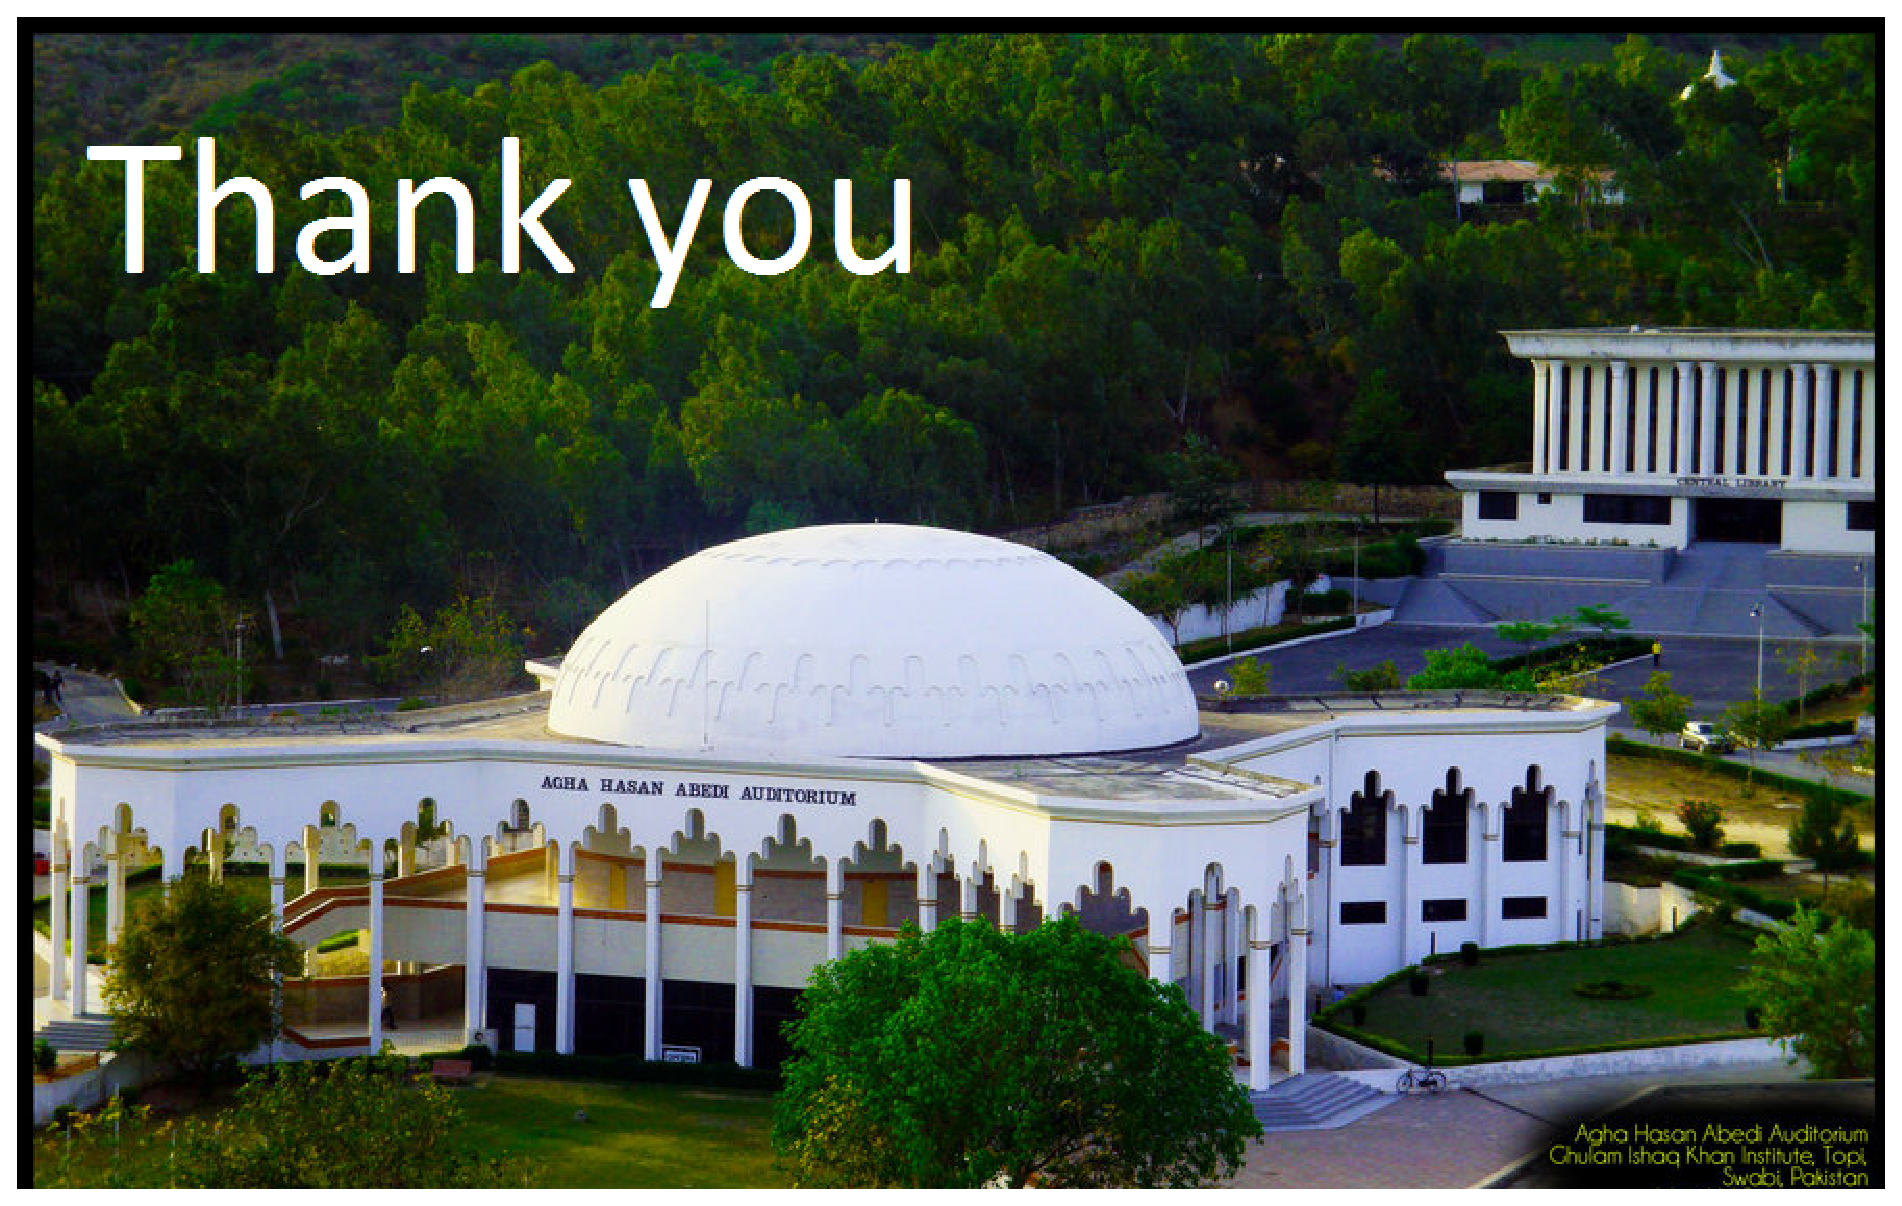
\includegraphics[width=0.99\textwidth]{GIK1.eps}\\
			%\caption{Plot for different values of $R_{e}$}\label{chF8}
		\end{figure}
	\end{frame}			
			
			
			
			
			
}	
	
	
	
	
	
	
	
	
	
	
	
	
	
	
	
\end{document}